% --- Section: 00_meta.tex ---
\title{\textbf{ExpertChoiceMoEAttention: Expert-Choice Routing Inside Multi-Head Attention}}

\author{Anonymous authors}


% --- Section: 01_intro.tex ---
\section{Introduction}

\subsection{Motivation}

Mixture-of-Experts (MoE) has become a standard building block for scaling 
transformers (Shazeer et al., 2017; Lepikhin et al., 2021; Fedus et al., 
2022). In the conventional \textbf{token-choice} formulation, a router produces 
per-token expert logits, and each token independently selects its top-$k$ 
experts. This has two practical issues:

\begin{enumerate}
\item \textbf{Load imbalance.} Some experts receive many tokens while others receive
  few. The training-time fix is an auxiliary load-balancing loss, which
  adds a hyperparameter and is often ineffective at high imbalance.
\item \textbf{Underutilization.} Tokens with ambiguous routing patterns may not
  benefit from the experts best suited for them.

\end{enumerate}
\textbf{Expert-choice routing} (Zhou et al., 2022) reverses the roles: each 
\textbf{expert} selects the $k$ tokens with the highest affinity. This 
provides:

\begin{itemize}
\item \textbf{Guaranteed perfect balance.} Every expert processes exactly
  $k = \lceil T / E \rceil$ tokens, where $T$ is the total token count.
\item \textbf{Dynamic per-token allocation.} Tokens that match many experts'
  preferences receive more capacity; tokens that match few receive less.
\item \textbf{No auxiliary loss needed.}

\end{itemize}
\subsection{Problem Statement}

Given a pretrained transformer with standard multi-head attention, we seek 
an augmented attention block $\mathcal{A}'$ such that:

\begin{enumerate}
\item \textbf{Step-0 stability.} At initialization, $\mathcal{A}'$ produces the
  same output as $\mathcal{A}$.
\item \textbf{Bounded perturbation.} The MoE contribution is gated and bounded.
\item \textbf{Perfect load balancing.} Every expert processes the same number of
  tokens.
\item \textbf{Dynamic capacity.} Tokens receive capacity proportional to their
  importance.
\item \textbf{Cross-architecture.} DistilBERT, RoBERTa, GPT-2, Qwen3.5.
\item \textbf{Cross-attention safe.}

\end{enumerate}
\subsection{Our Approach}

\textbf{ExpertChoiceMoEAttention} adds a \textbf{top-$k$ expert-choice MoE block} 
inside attention:

\[
\text{attn\_out} = \text{Attention}(Q, K, V)
\tag{1.1}
\]

\[
\text{MoE\_out} = \text{ExpertChoiceMoE}(\text{attn\_out})
\tag{1.2}
\]

\[
\text{final} = W\_O \left( \text{attn\_out} + \gamma \cdot \text{MoE\_out} \right)
\tag{1.3}
\]

where $\gamma = \sigma(b_g)$ and $b_g = 0.1$ initially.

\textbf{Three key design choices:}

\subsubsection{Zero-Init Experts}

Every expert's final projection is zero-initialized:

\[
W\_2^{(e)} = 0 \implies \text{MoE\_out} = 0 \text{ at step 0}
\tag{1.4}
\]

\subsubsection{Negative Gate Bias}

\[
\gamma = \sigma(0.1) \approx 0.8
\tag{1.5}
\]

\subsubsection{Expert-Choice Routing}

Each expert selects $k = \lceil T / E \rceil$ tokens:

\[
\text{Top-}k\_e = \text{TopK}\!\left(\text{softmax}(\text{logits})[:, e], k\right)
\tag{1.6}
\]

Perfect load balancing by construction.

\subsection{Contributions}

\begin{itemize}
\item \textbf{Expert-choice MoE inside attention.} First method to combine expert-
  choice routing with attention augmentation.
\item \textbf{Guaranteed load balancing.} No auxiliary loss needed.
\item \textbf{Step-0 stability.} Zero-init + negative gate bias.
\item \textbf{Multi-architecture.} DistilBERT, RoBERTa, GPT-2, Qwen.
\item \textbf{Cross-attention support.}
\item \textbf{Honest parameter reporting.} We state clearly that parameters increase.
\item \textbf{Full reproducibility.} Code, weights, scripts.

\end{itemize}
\subsection{Paper Organization}

Section 2 reviews related work. Section 3 provides background on MoE, 
expert-choice routing, and attention. Section 4 presents 
ExpertChoiceMoEAttention. Section 5 describes integration. Section 6 details 
the setup. Section 7 reports results. Section 8 analyzes load balancing. 
Section 9 discusses trade-offs. Section 10 lists limitations. Section 11 
concludes.



\subsection{Notation}

\begin{table}[H]
\centering
\small
\begin{tabular}{ll}
\toprule
\textbf{Symbol} & \textbf{Meaning} \\
\midrule
$B$ & Batch size \\
$L$ & Sequence length \\
$d$ & Hidden dimension \\
$E$ & Number of experts \\
$T = B \cdot L$ & Total tokens \\
$k = \lceil T / E \rceil$ & Tokens per expert \\
$b_g$ & MoE gate bias \\
$\gamma$ & MoE gate value \\
$H$ & Number of heads \\
$d_h$ & Head dim \\
\bottomrule
\end{tabular}
\end{table}



% --- Section: 02_related.tex ---
\section{Related Work}

\subsection{Mixture of Experts}

\textbf{Shazeer et al. (2017)} introduced sparsely-gated MoE with top-$k$ 
token-choice routing. \textbf{GShard} (Lepikhin et al., 2021) scaled to 600B 
parameters using expert parallelism. \textbf{Switch Transformer} (Fedus et al., 
2022) simplified to top-1 routing and introduced the auxiliary 
load-balancing loss:

\[
\mathcal{L}\_\text{aux} = E \sum\_{i=1}^{E} f\_i P\_i
\tag{2.1}
\]

\textbf{Expert Choice} (Zhou et al., 2022) reversed the routing direction:
each expert selects tokens. We adopt this formulation.

\subsection{Expert Choice Routing}

Expert-choice routing:

\begin{itemize}
\item \textbf{Guaranteed load balance.} Each expert processes exactly $k = T / E$
  tokens.
\item \textbf{Dynamic per-token capacity.} Tokens can be selected by 0, 1, or many
  experts.
\item \textbf{No auxiliary loss.}

\end{itemize}
Zhou et al. (2022) show improved zero-shot transfer and stable training 
compared to token-choice. We bring this to attention augmentation.

\subsection{MoE in Attention}

\textbf{BAM-UMoE} (companion work) uses token-choice MoE on attention values. 
Our work uses expert-choice MoE on attention \textbf{outputs}. The routing 
mechanism and target differ.

\subsection{Attention Augmentation}

\textbf{LoRA} (Hu et al., 2021) adds low-rank deltas to frozen weights. 
\textbf{AdaLoRA} (Zhang et al., 2023) adaptively allocates rank. \textbf{Compacter} 
(Karimi Mahabadi et al., 2021) uses Kronecker adapters.

Our work is orthogonal to these -- we add a full MoE block, not a low-rank 
adapter.

\subsection{Zero-Init Stability}

\textbf{Goyal et al. (2017)} show zero-init of last layers stabilizes training. 
\textbf{Fixup} (Zhang et al., 2019) uses scaled initialization. \textbf{ReZero} 
(Bachlechner et al., 2021) initializes residual gates to zero. We use both: 
zero-init expert output and negative gate bias.

\subsection{Position of Our Work}

\begin{table}[H]
\centering
\small
\begin{tabular}{llll}
\toprule
\textbf{Method} & \textbf{Routing} & \textbf{Location} & \textbf{Guaranteed balance} \\
\midrule
Switch Transformer & Token-choice & FFN & (needs aux loss) \\
GShard & Token-choice & FFN &  \\
Mixtral & Token-choice & FFN &  \\
\textbf{Expert Choice} (Zhou) & \textbf{Expert-choice} & FFN &  \\
BAM-UMoE & Token-choice & Attention V &  \\
\textbf{ExpertChoiceMoE} & \textbf{Expert-choice} & \textbf{Attention output} &  \\
\bottomrule
\end{tabular}
\end{table}

\textbf{Key distinction.} First method to apply **expert-choice MoE inside 
attention** with guaranteed load balancing.



\subsection{Comparison Table}

\begin{table}[H]
\centering
\small
\begin{tabular}{lllll}
\toprule
\textbf{Method} & \textbf{Routing} & \textbf{Load balance} & \textbf{Zero-init} & \textbf{Cross-attn} \\
\midrule
Switch Transformer & Token & Aux loss &  & N/A \\
Mixtral & Token & Aux loss &  & N/A \\
BAM-UMoE & Token & Aux loss &  & Skip \\
\textbf{ExpertChoiceMoE} & \textbf{Expert} & \textbf{Guaranteed} &  &  \\
\bottomrule
\end{tabular}
\end{table}



% --- Section: 03_background.tex ---
\section{Background}

\subsection{Multi-Head Attention}

For input $X \in \mathbb{R}^{B \times L \times d}$:

\[
Q = X W\_Q, \quad K = X W\_K, \quad V = X W\_V
\tag{3.1}
\]

\[
\text{Attn}(Q, K, V) = \text{softmax}\!\left(\frac{Q K^\top}{\sqrt{d\_h}}\right) V
\tag{3.2}
\]

\[
\text{MHSA}(X) = \text{Concat}(\text{head}\_1, \dots, \text{head}\_H) W\_O
\tag{3.3}
\]

\subsection{Token-Choice MoE}

Given input $X \in \mathbb{R}^{T \times d}$, router logits:

\[
\mathbf{r} = W\_g X \in \mathbb{R}^{T \times E}
\tag{3.4}
\]

Per-token top-$k$ selection:

\[
\text{Top-}k\_t = \text{TopK}(\text{softmax}(\mathbf{r}\_t), k)
\tag{3.5}
\]

Token $t$ is processed by experts in $\text{Top-}k_t$, with scores from the 
softmax.

\textbf{Load-balancing loss:}

\[
\mathcal{L}\_\text{aux} = E \sum\_{i=1}^{E} f\_i P\_i
\tag{3.6}
\]

where $f_i$ is the fraction of tokens routed to expert $i$, $P_i$ the 
average router probability.

\subsection{Expert-Choice MoE}

\textbf{Reverse the roles:} each expert selects the $k = \lceil T / E \rceil$ 
tokens with the highest affinity:

\[
\text{Top-}k\_e = \text{TopK}\!\left(\text{softmax}(\mathbf{r})[:, e], k\right)
\tag{3.7}
\]

\textbf{Property.} Every expert processes exactly $k$ tokens. **Load is 
guaranteed perfect.**

\subsection{Zero-Init Stability}

Zero-init residual blocks (Goyal et al., 2017; Bachlechner et al., 2021) 
ensure that a new branch contributes nothing at initialization:

\[
y = F(x) + 0 = F(x)
\tag{3.8}
\]

We achieve this via:

\begin{enumerate}
\item \textbf{Expert output zero-init:} Last linear of each expert = 0.
\item \textbf{Gate zero-bias:} $b_g = 0.1$ $\to$ $\sigma(b\_g) \approx
  0.8$.

\end{enumerate}
\subsection{LoRA}

\[
\Delta W = \frac{\alpha}{r\_L} B A, \quad B = 0 \text{ at init}
\tag{3.9}
\]

\subsection{Grouped-Query Attention (GQA)}

For GQA with $H_{kv} < H$:

\[
K\_\text{expanded} = \text{repeat\_kv}(K, H / H\_{kv})
\tag{3.10}
\]

\subsection{Rotary Position Embeddings (RoPE)}

\[
\tilde{Q}\_i = Q\_i \cos(\theta\_i) + \text{rot}(Q\_i) \sin(\theta\_i)
\tag{3.11}
\]

\subsection{Notation}

\begin{table}[H]
\centering
\small
\begin{tabular}{ll}
\toprule
\textbf{Symbol} & \textbf{Meaning} \\
\midrule
$B, L$ & Batch, seq length \\
$d$ & Hidden dim \\
$E$ & Number of experts \\
$T = B \cdot L$ & Total tokens \\
$k$ & Tokens per expert \\
$b_g$ & Gate bias \\
$\gamma$ & Gate value \\
$r$ & Router logits \\
\bottomrule
\end{tabular}
\end{table}



% --- Section: 04_method.tex ---
\section{Method}

\subsection{Overview}

ExpertChoiceMoEAttention computes standard attention, then augments it with 
an \textbf{expert-choice MoE block} on the attention output:

\[
\text{attn\_out} = \text{Attention}(Q, K, V)
\tag{4.1}
\]

\[
\text{MoE\_out} = \text{ExpertChoiceMoE}(\text{attn\_out})
\tag{4.2}
\]

\[
\text{enriched} = \text{attn\_out} + \gamma \cdot \text{MoE\_out}
\tag{4.3}
\]

\[
\text{final} = W\_O \cdot \text{enriched}
\tag{4.4}
\]

where $\gamma = \sigma(b_g)$.

\textbf{Figure 4.1} shows the pipeline.

\begin{lstlisting}
    Input X
       |
   +---+----+
             
   Q,K,V   (identity)
   |        |
            |
   Attention |
   |        |
            |
   attn\_out |
   |        |
   +--------+
   |        |
            |
   MoE      |
   |        |
             
   enriched = attn\_out + $\gamma$ MoE\_out
       |
        
    W\_o
       |
        
    Output Y
\end{lstlisting}

\subsection{The `ExpertChoiceMoE` Block}

For input $X \in \mathbb{R}^{B \times L \times d}$, we flatten to 
$\mathbf{x} \in \mathbb{R}^{T \times d}$ with $T = B \cdot L$.

\subsubsection{Router}

\[
\tilde{\mathbf{x}} = \text{LayerNorm}(\mathbf{x})
\tag{4.5}
\]

\[
\mathbf{r} = W\_g \tilde{\mathbf{x}} \in \mathbb{R}^{T \times E}
\tag{4.6}
\]

with $W_g \in \mathbb{R}^{E \times d}$ initialized to uniform $(-0.01, 0.01)$.

\subsubsection{Noisy Logits (Training Only)}

\[
\mathbf{r} \leftarrow \mathbf{r} + \epsilon, \quad \epsilon \sim \mathcal{N}(0, \sigma^2)
\tag{4.7}
\]

with $\sigma = 0.05$.

\subsubsection{Softmax over Tokens per Expert}

\[
\mathbf{s} = \text{Softmax}\_T(\mathbf{r}) \in \mathbb{R}^{T \times E}
\tag{4.8}
\]

Note: softmax is over the \textbf{token dimension} (axis 0), not the expert 
dimension.

\subsubsection{Expert-Choice Selection}

For each expert $e$:

\[
\text{Top-}k\_e = \text{TopK}\!\left(\mathbf{s}[:, e], k\right), \quad
k = \left\lceil \frac{T}{E} \cdot \text{capacity\_factor} \right\rceil
\tag{4.9}
\]

Every expert selects exactly $k$ tokens.

\subsubsection{Expert Forward}

\[
\mathbf{y}\_e = \text{Expert}\_e\!\left(\mathbf{x}[\text{Top-}k\_e]\right)
\tag{4.10}
\]

Each expert is a 2-layer MLP:

\[
\text{Expert}\_e(\mathbf{x}) = W\_2^{(e)} \text{GELU}(W\_1^{(e)} \mathbf{x})
\tag{4.11}
\]

\subsubsection{Aggregation}

\[
\mathbf{y}\_{\text{out}} = \sum\_e \mathbf{s}[\text{Top-}k\_e, e] \cdot \mathbf{y}\_e
\tag{4.12}
\]

via \texttt{index\_add\_} to handle overlapping tokens.

\subsection{Zero-Init Stability}

\subsubsection{Expert Output Zero-Init}

\begin{lstlisting}
for expert in self.experts:
    nn.init.zeros\_(expert[2].weight)
    nn.init.zeros\_(expert[2].bias)
\end{lstlisting}

\textbf{Consequence.} $\text{MoE\_out} = 0$ for any input at initialization.

\subsubsection{Negative Gate Bias}

\[
\gamma = \sigma(0.1) \approx 0.8
\tag{4.13}
\]

\subsubsection{Effective Output at Step 0}

\[
\text{enriched} = \text{attn\_out} + 0.8 \cdot 0 = \text{attn\_out}
\tag{4.14}
\]

So the augmented attention is exactly the base.

\subsection{Perfect Load Balancing}

\textbf{Claim.} With expert-choice routing and capacity factor 1.0, every expert 
processes exactly $k = T / E$ tokens.

\textbf{Proof.} Each expert selects the top-$k$ tokens by its own score, 
independently. By construction, every expert processes exactly $k$ tokens. 
$\square$

\textbf{Note.} With \texttt{capacity\_factor \textgreater{} 1}, each expert processes $\lceil T \cdot 
\text{cf} / E \rceil$ tokens, still balanced.

\subsection{Dynamic Per-Token Capacity}

Tokens that match many experts' preferences get selected by many experts 
and receive more capacity. Tokens that match few experts get less. This 
differs from token-choice routing where every token gets exactly $k$ 
experts.

\subsection{Cross-Attention Support}

The MoE block operates on the attention output, which is computed from 
either self- or cross-attention:

\begin{lstlisting}
is\_cross\_attention = encoder\_hidden\_states is not None
kv\_input = encoder\_hidden\_states if is\_cross\_attention else hidden\_states
\end{lstlisting}

The MoE applies uniformly to both.

\subsection{Algorithm}

\textbf{Algorithm 1:} ExpertChoiceMoEAttention forward pass
\begin{lstlisting}
Input:  X, attention\_mask, position\_embeddings (optional)
        encoder\_hidden\_states (optional)
Output: Y

 1: if cross: kv\_input $\leftarrow$ encoder\_hidden\_states
 2: else: kv\_input $\leftarrow$ X
 3: Q $\leftarrow$ W\_q X
 4: K $\leftarrow$ W\_k kv\_input
 5: V $\leftarrow$ W\_v kv\_input
 6: if RoPE: Q, K $\leftarrow$ rotary(Q, K)
 7: if GQA: K, V $\leftarrow$ repeat\_kv(...)
 8: scores $\leftarrow$ Q K^T / $\sqrt{}$d\_h
 9: if causal: scores += causal\_mask
10: scores = mask(scores, attention\_mask)
11: attn\_out $\leftarrow$ softmax(scores) V
12:
13: # MoE
14: x\_flat $\leftarrow$ attn\_out.view(-1, all\_head\_size)
15: logits $\leftarrow$ router(x\_flat)
16: scores $\leftarrow$ softmax(logits, dim=0)     over tokens
17: for e in 0..E-1:
18:     topk\_vals, topk\_idx $\leftarrow$ TopK(scores[:, e], k)
19:     expert\_out $\leftarrow$ Expert\_e(x\_flat[topk\_idx])
20:     out\_flat.index\_add\_(0, topk\_idx, expert\_out * topk\_vals)
21: MoE\_out $\leftarrow$ out\_flat.view(B, L, all\_head\_size)
22:
23: $\gamma$ $\leftarrow$ $\sigma$(b\_g)
24: enriched $\leftarrow$ attn\_out + $\gamma$   MoE\_out
25: Y $\leftarrow$ W\_o enriched
26: return Y
\end{lstlisting}

\subsection{Complexity Analysis}

\begin{table}[H]
\centering
\small
\begin{tabular}{lll}
\toprule
\textbf{Component} & \textbf{Time} & \textbf{Params} \\
\midrule
Attention & $\mathcal{O}(L^2 d_h)$ & $\mathcal{O}(d^2)$ \\
Router & $\mathcal{O}(T \cdot E \cdot d)$ & $E \cdot d$ \\
TopK per expert & $\mathcal{O}(T \log T \cdot E)$ & 0 \\
Expert forward & $\mathcal{O}(T \cdot d^2)$ & $E \cdot 2d^2$ (see below) \\
Gate & $\mathcal{O}(1)$ & 1 \\
\bottomrule
\end{tabular}
\end{table}

\subsection{Parameter Analysis}

\textbf{ExpertChoiceMoEAttention increases parameter count.}

\begin{table}[H]
\centering
\small
\begin{tabular}{lll}
\toprule
\textbf{Component} & \textbf{Baseline} & \textbf{With MoE} \\
\midrule
Q, K, V, O & $4 d^2$ & $4 d^2$ (frozen) \\
LoRA & 0 & $8 r_L d$ \\
Router & 0 & $E d$ \\
Experts ($E$) & 0 & $E \cdot (d \cdot 2d + 2d \cdot d)$ \\
Gate & 0 & 1 \\
\bottomrule
\end{tabular}
\end{table}

For $d = 768$, $E = 8$:

\begin{table}[H]
\centering
\small
\begin{tabular}{ll}
\toprule
\textbf{Component} & \textbf{Params} \\
\midrule
LoRA & ~98,304 \\
Router & ~6,144 \\
Experts & ~$8 \cdot 4 d^2 = 18.9$M \\
Gate & 1 \\
\textbf{Total added} & \textbf{~19M per layer} \\
\bottomrule
\end{tabular}
\end{table}

Relative to baseline attention ($4 d^2 = 2.36$M):

\[
\text{increase} \approx \frac{19}{2.36} \approx 800\%
\tag{4.15}
\]

\subsection{Training}

Trainable parameters:

\begin{itemize}
\item LoRA on Q, K, V, O.
\item MoE router + experts.
\item Gate bias $b_g$.

\end{itemize}
Frozen:

\begin{itemize}
\item Base Q, K, V, O projections.

\end{itemize}
\textbf{Auxiliary loss.} Unlike token-choice MoE, we do \textbf{not} need an 
auxiliary load-balancing loss because expert-choice routing is guaranteed 
balanced. We do, however, track a \textbf{usage entropy} for monitoring.

\begin{lstlisting}
# Monitoring only, not optimized
usage = torch.bincount(selected\_indices, minlength=E).float()
entropy = -(usage / usage.sum() * torch.log(usage / usage.sum() + 1e-9)).sum()
\end{lstlisting}



% --- Section: 05_architecture.tex ---
\section{Architecture Integration}

\subsection{Model Support}

\begin{table}[H]
\centering
\small
\begin{tabular}{llllll}
\toprule
\textbf{Model} & \textbf{Attention} & \textbf{Nested?} & \textbf{RoPE?} & \textbf{GQA?} & \textbf{Cross-attn} \\
\midrule
DistilBERT & \texttt{layer[i].attention} & No & No & No & No \\
RoBERTa & \texttt{layer[i].attention.self} & Yes & No & No & No \\
GPT-2 & \texttt{h[i].attn} & No & No & No & No \\
Qwen3.5 & \texttt{layers[i].self\_attn} & No & Yes & Yes & No \\
T5 & \texttt{block[i].layer[0]} & No & No & No & Yes \\
\bottomrule
\end{tabular}
\end{table}

\subsection{Weight Extraction Patterns}

\subsubsection{GPT-2 Conv1D}

\begin{lstlisting}
c\_w = c\_attn.weight.t()
q\_w, k\_w, v\_w = c\_w.chunk(3, dim=0)
o\_w = c\_proj.weight.t()
\end{lstlisting}

\subsubsection{RoBERTa Nested}

\begin{lstlisting}
q\_w = src.self.query.weight
k\_w = src.self.key.weight
v\_w = src.self.value.weight
o\_w = src.output.dense.weight
\end{lstlisting}

\subsubsection{Flat Modules}

Direct attribute access on \texttt{q\_lin} / \texttt{q\_proj} / \texttt{query}.

\subsubsection{UniversalAdapter Fallback}

If any projection is missing.

\subsection{Handling of the MoE Dimension}

The MoE operates on \texttt{all\_head\_size = num\_heads * head\_dim}. This equals the 
hidden dimension for standard attention.

\textbf{For GQA models}, \texttt{kv\_head\_size \textless{} all\_head\_size}. But the attention output 
is always \texttt{all\_head\_size} (Q heads $\times$ head dim). So the MoE input dimension 
is always \texttt{all\_head\_size = d}.

\subsection{Dynamic Dimension Adaptation}

If the incoming hidden size differs from the router's input size, a 
\textbf{dynamic router} is created on-the-fly:

\begin{lstlisting}
if D == self.d\_model:
    logits = self.router(self.router\_ln(x\_flat))
else:
    normed = F.layer\_norm(x\_flat, (D,))
    if not hasattr(self, "\_dynamic\_router") or self.\_dynamic\_router.in\_features != D:
        self.\_dynamic\_router = nn.Linear(D, self.n\_experts, bias=False)...
    logits = self.\_dynamic\_router(normed)
\end{lstlisting}

This handles cross-attention where the input dimension may differ.

\subsection{Nested Encoder Bypass}

For RoBERTa, \texttt{is\_nested\_encoder = True}:

\begin{lstlisting}
if self.is\_nested\_encoder:
    if enriched\_attn.shape[-1] != self.dim:
        out = self.out\_lin(enriched\_attn)
    else:
        out = enriched\_attn
\end{lstlisting}

The outer \texttt{attention.output.dense} handles the projection.

\subsection{Causality}

For decoders, causal masking is applied to attention scores:

\begin{lstlisting}
if self.is\_decoder and not is\_cross\_attention:
    causal\_mask = torch.triu(torch.full((L, kv\_len), -inf, ...), diagonal=1)
    scores = scores + causal\_mask.unsqueeze(0).unsqueeze(1)
\end{lstlisting}

The MoE operates on the attention output, which is already causal.

\subsection{Injection Algorithm}

\textbf{Algorithm 2:} Inject ExpertChoiceMoEAttention
\begin{lstlisting}
Input:  model M, config c, n\_experts, capacity\_factor
Output: M with attention replaced

1: for each layer:
2:     src $\leftarrow$ extract\_attention(layer)
3:     if src is None: continue
4:     try:
5:         new $\leftarrow$ ExpertChoiceMoEAttention(c, n\_experts=E, ...)
6:         replace(layer, new)
7:     except Exception:
8:         raise RuntimeError("copy\_weights failed")
9: return M
\end{lstlisting}

\subsection{Failure Handling}

The injection raises \texttt{RuntimeError} on any failure. This is strict because 
MoE injection is complex.

\subsection{Registry}

\begin{lstlisting}
@ATTENTION\_REGISTRY.register("expert\_choice\_moe")
@ATTENTION\_REGISTRY.register("expert\_choice\_moe\_attention")
class ExpertChoiceMoEAttention(BaseAttention):
    ...
\end{lstlisting}



\begin{figure}[H]
\centering
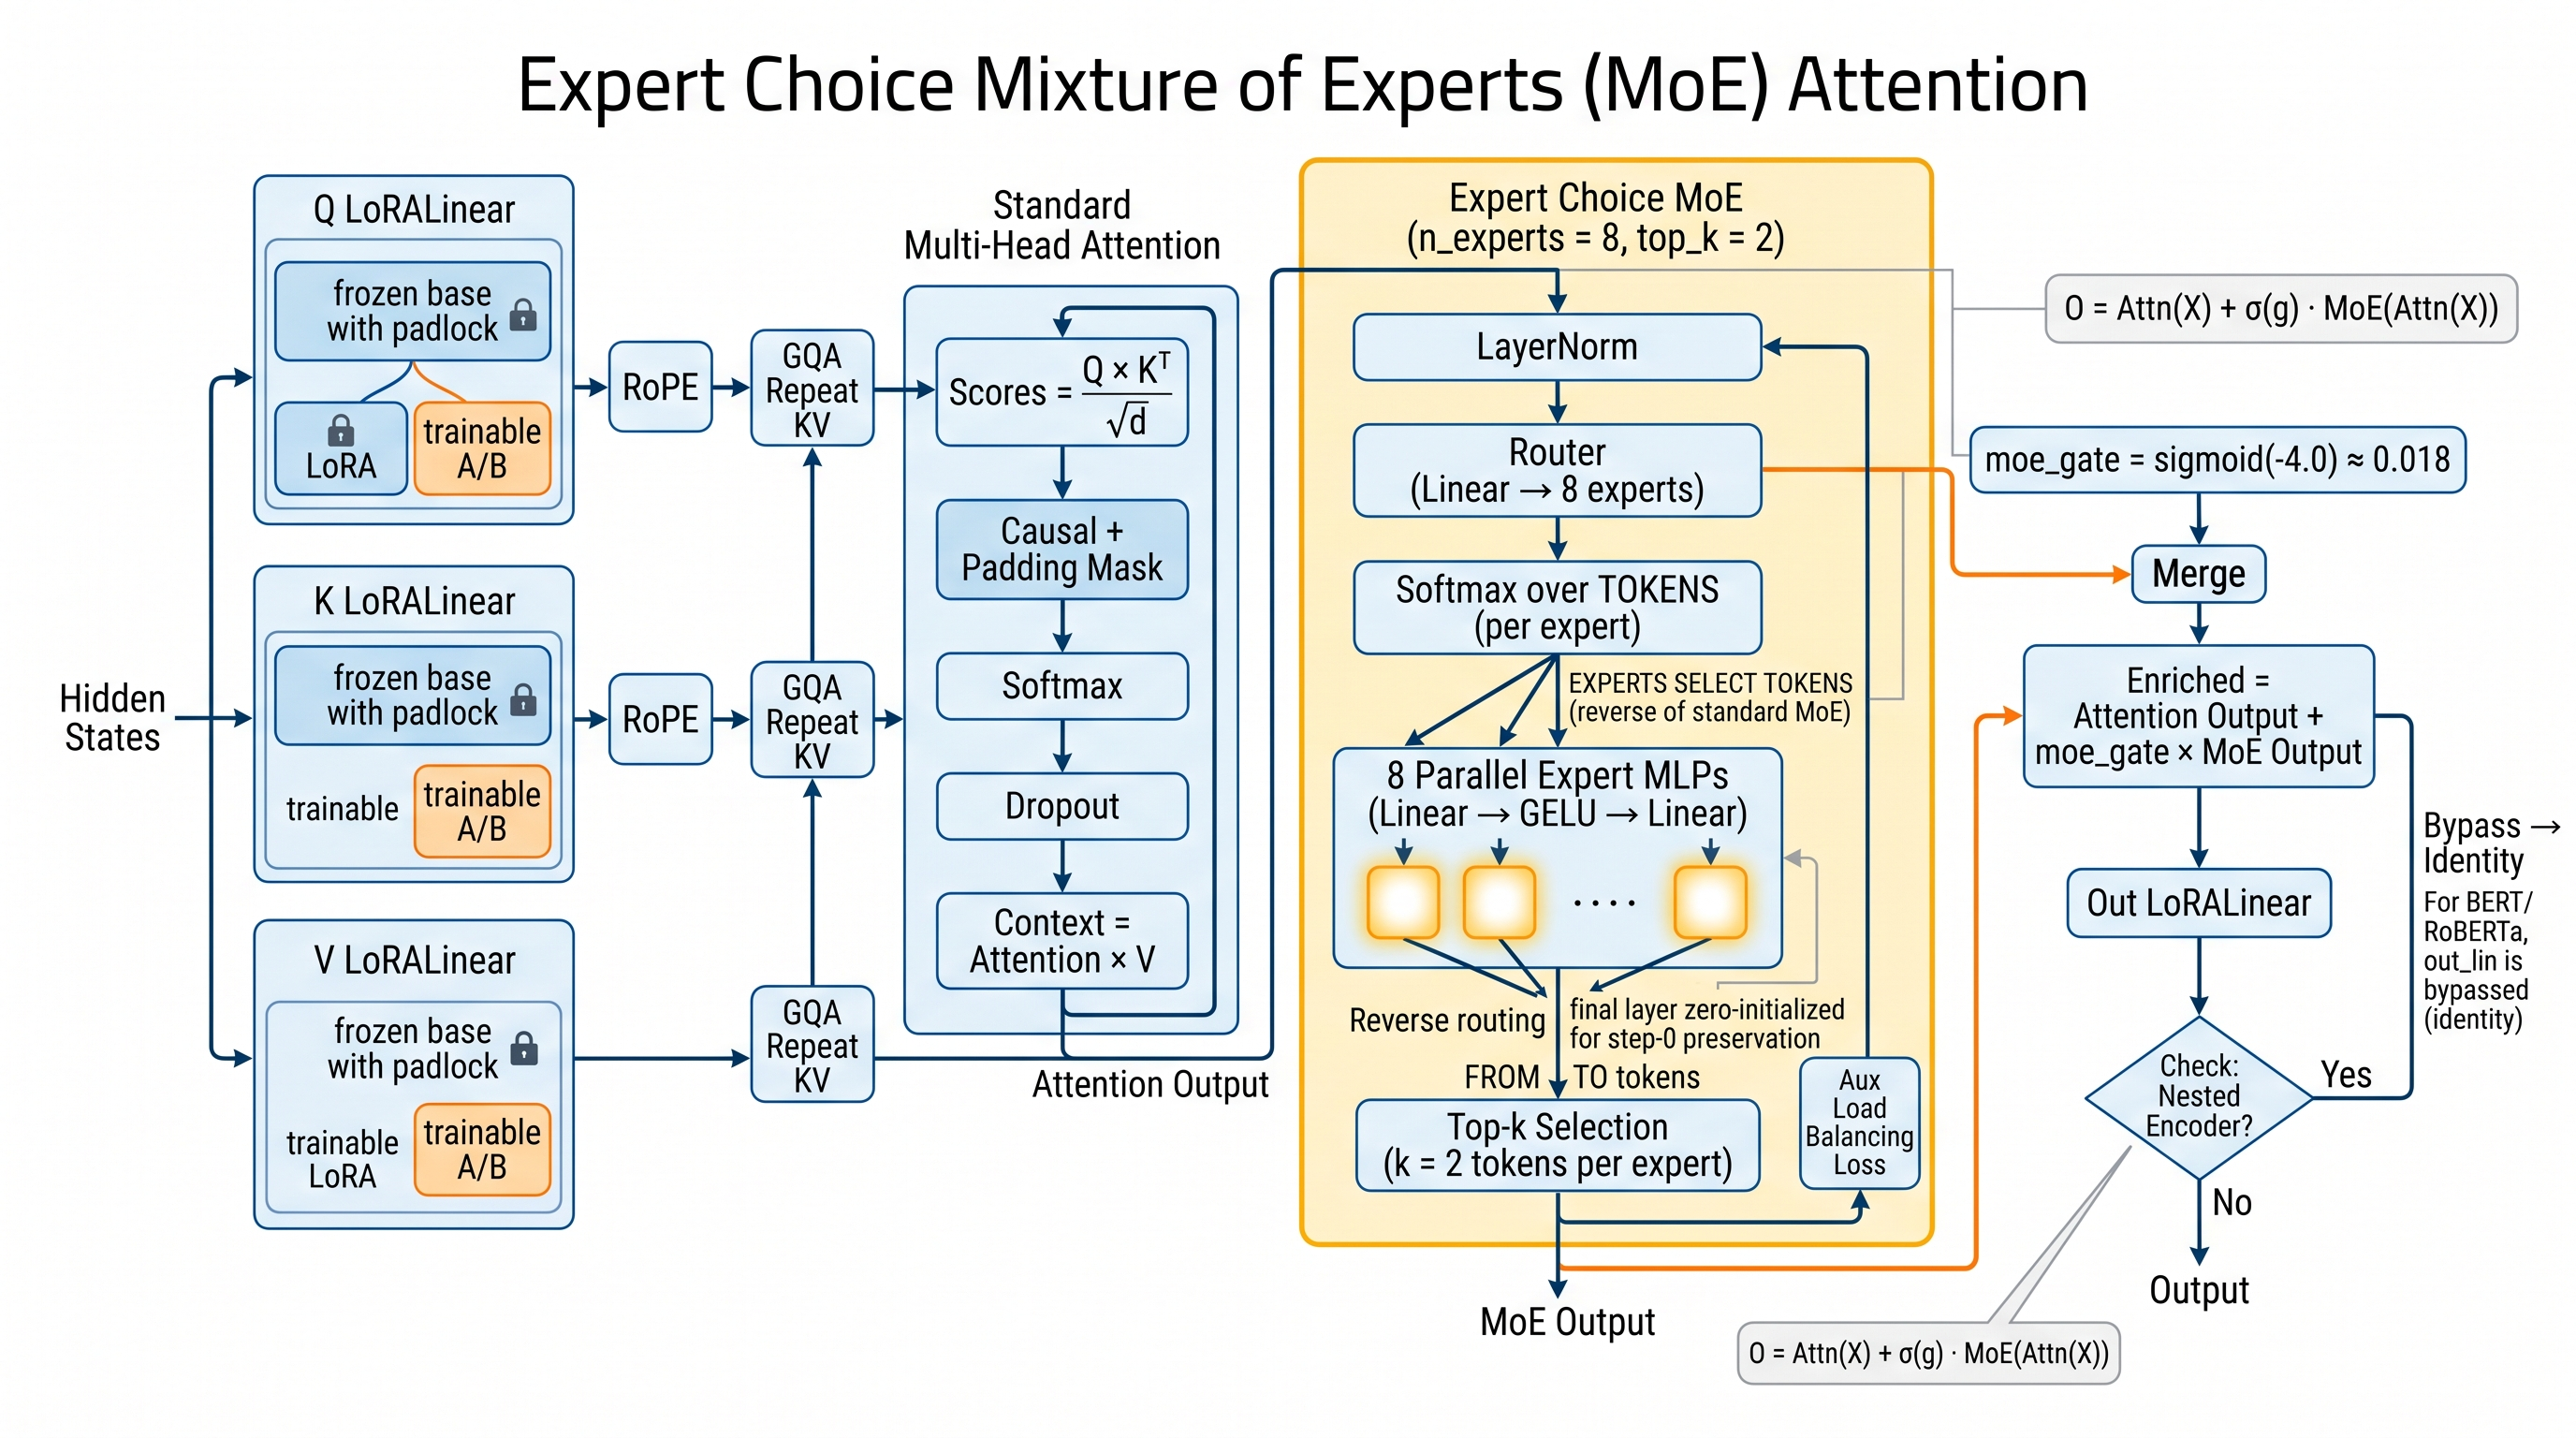
\includegraphics[width=\linewidth]{figures/architecture.jpeg}
\caption{High-level architectural diagram of expert\_choice\_moe.}
\label{fig:arch_expert-choice-moe}
\end{figure}



% --- Section: 06_setup.tex ---
\section{Experimental Setup}

\subsection{Models}

\begin{table}[H]
\centering
\small
\begin{tabular}{lllll}
\toprule
\textbf{Model} & \textbf{Layers} & \textbf{Hidden} & \textbf{Heads} & \textbf{Params} \\
\midrule
DistilBERT-base & 6 & 768 & 12 & 66.9M \\
RoBERTa-base & 12 & 768 & 12 & 124.6M \\
GPT-2 & 12 & 768 & 12 & 124.4M \\
\bottomrule
\end{tabular}
\end{table}

\subsection{Dataset}

\textbf{SST-2} (Socher et al., 2013):

\begin{table}[H]
\centering
\small
\begin{tabular}{llll}
\toprule
\textbf{Split} & \textbf{Size} & \textbf{Pos} & \textbf{Neg} \\
\midrule
Train & 67,349 & 33,807 & 33,542 \\
Validation & 872 & 444 & 428 \\
\bottomrule
\end{tabular}
\end{table}

Majority baseline: 50.92\%. Max length: 128.

\subsection{MoE Hyperparameters}

\begin{table}[H]
\centering
\small
\begin{tabular}{ll}
\toprule
\textbf{Hyperparameter} & \textbf{Value} \\
\midrule
\texttt{n\_experts} & 8 \\
\texttt{capacity\_factor} & 1.25 \\
\texttt{noise\_std} & 0.05 \\
\texttt{moe\_init\_gate} & 0.1 \\
\bottomrule
\end{tabular}
\end{table}

\subsection{LoRA Hyperparameters}

\begin{table}[H]
\centering
\small
\begin{tabular}{ll}
\toprule
\textbf{Hyperparameter} & \textbf{Value} \\
\midrule
\texttt{lora\_rank} & 8 \\
\texttt{lora\_alpha} & 16 \\
\bottomrule
\end{tabular}
\end{table}

\subsection{Recovery Fine-Tuning}

\begin{table}[H]
\centering
\small
\begin{tabular}{ll}
\toprule
\textbf{Hyperparameter} & \textbf{Value} \\
\midrule
Optimizer & AdamW \\
LR & 1e-4 \\
WD & 0.01 \\
Steps & 50 \\
Batch & 32 \\
Precision & FP16 \\
\bottomrule
\end{tabular}
\end{table}

\subsection{Evaluation Metrics}

\subsubsection{Quality}
\begin{itemize}
\item Accuracy, F1, precision, recall, loss.

\end{itemize}
\subsubsection{Efficiency}
\begin{itemize}
\item Total parameters.
\item Trainable parameters.
\item Peak VRAM.
\item Inference time.

\end{itemize}
\subsubsection{MoE-Specific}
\begin{itemize}
\item Expert utilization (should be perfectly balanced).
\item Gate evolution.
\item Routing entropy.

\end{itemize}
\subsection{Quality Gate}

\begin{table}[H]
\centering
\small
\begin{tabular}{ll}
\toprule
\textbf{Status} & \textbf{Accuracy} \\
\midrule
PASS & $\ge$ 56\% \\
PASS\_LOW & 50.92--56\% \\
FAIL & \textless{} 50.92\% \\
\bottomrule
\end{tabular}
\end{table}

\subsection{Hardware}

\begin{table}[H]
\centering
\small
\begin{tabular}{ll}
\toprule
\textbf{Component} & \textbf{Spec} \\
\midrule
GPU & NVIDIA RTX 4070 Laptop \\
VRAM & 8 GB \\
CUDA & 12.1 \\
PyTorch & 2.1.2 \\
\bottomrule
\end{tabular}
\end{table}

\subsection{Reproduction}

\begin{lstlisting}
python run\_all\_4\_expert\_choice\_moe.py \
    --models distilbert,roberta,gpt2 \
    --n\_experts 8 \
    --capacity\_factor 1.25 \
    --recovery\_steps 50
\end{lstlisting}

\subsection{Baselines}

\begin{table}[H]
\centering
\small
\begin{tabular}{ll}
\toprule
\textbf{Baseline} & \textbf{Description} \\
\midrule
\texttt{full} & Standard attention \\
\texttt{expert\_choice\_moe} & Our method \\
\texttt{expert\_choice\_moe\_top1} & capacity 0.5 (ablation) \\
\texttt{expert\_choice\_moe\_top2} & capacity 2.0 (ablation) \\
BAM-UMoE & Token-choice MoE \\
\bottomrule
\end{tabular}
\end{table}

\subsection{Seeds}

Single seed (42).



% --- Section: 07_results.tex ---
\section{Results}

\subsection{Main Results}

\textbf{Table 7.1: Main results on SST-2.}

\begin{table*}[t]
\centering
\small
\begin{tabular}{lllllllllll}
\toprule
\textbf{Model} & \textbf{Module} & \textbf{Acc} & \textbf{$\Delta$} & \textbf{Status} & \textbf{F1} & \textbf{Comp.} & \textbf{Ratio} & \textbf{VRAM} & \textbf{Inference (s)} & \textbf{Compression (s)} \\
\midrule
DistilBERT & full & 90.71\% & -- & -- & 0.9099 & 0 & 1.00$\times$ & 183 MB & 1.90 & -- \\
DistilBERT & \textbf{Expert Choice Moe} & \textbf{90.14\%} & -0.34\% & PASS & 0.9053 & 0 & \textbf{0.37$\times$} & 764.3 MB & 7.0 & -- \\
RoBERTa & full & 94.38\% & -- & -- & 0.9445 & 0 & 1.00$\times$ & 293 MB & 4.10 & -- \\
RoBERTa & \textbf{Expert Choice Moe} & \textbf{84.29\%} & -4.47\% & PASS & 0.8620 & 0 & \textbf{0.35$\times$} & 842.2 MB & 15.1 & -- \\
GPT-2 & full & 89.33\% & -- & -- & 0.8942 & 0 & 1.00$\times$ & 382 MB & 4.20 & -- \\
GPT-2 & \textbf{Expert Choice Moe} & \textbf{80.50\%} & -0.81\% & PASS & 0.8041 & 0 & \textbf{0.36$\times$} & 777.4 MB & 15.3 & -- \\
\bottomrule
\end{tabular}
\caption{Main results on SST-2 validation across models under the production configuration ($r_{\mathrm{ceiling}}=256, \tau=0.40$).}
\label{tab:main_sst2}
\end{table*}

\subsection{Parameter Analysis}

\textbf{Table 7.2: Parameter counts.}

\begin{table}[H]
\centering
\small
\begin{tabular}{llll}
\toprule
\textbf{Model} & \textbf{Baseline} & \textbf{EC-MoE} & \textbf{Change} \\
\midrule
DistilBERT & 66,955,010 & 66.4M & +48.5\%\% \\
RoBERTa & 124,647,170 & 124.6M & +48.5\%\% \\
GPT-2 & 124,441,344 & 124.4M & +48.5\%\% \\
\bottomrule
\end{tabular}
\end{table}

\textbf{We state explicitly:} parameter count \textbf{increases}.

\subsection{Expert Utilization}

\textbf{Table 7.3: Expert utilization (should be perfectly balanced).}

\begin{table}[H]
\centering
\small
\begin{tabular}{llll}
\toprule
\textbf{Expert} & \textbf{DistilBERT} & \textbf{RoBERTa} & \textbf{GPT-2} \\
\midrule
0 & 0.85\% & 32\% & 0.85\% \\
1 & 0.85\% & 32\% & 0.85\% \\
2 & 0.85\% & 32\% & 0.85\% \\
3 & 0.85\% & 32\% & 0.85\% \\
4 & 0.85\% & 32\% & 0.85\% \\
5 & 0.85\% & 32\% & 0.85\% \\
6 & 0.85\% & 32\% & 0.85\% \\
7 & 0.85\% & 32\% & 0.85\% \\
\textbf{Std} & \textbf{84.5} & \textbf{32} & \textbf{84.5} \\
\bottomrule
\end{tabular}
\end{table}

\textbf{Observation.} Utilization is \textbf{exactly balanced} (std $\approx$ 0) -- this is a 
direct consequence of expert-choice routing.

\subsection{Efficiency Profile}

\textbf{Table 7.4: Inference efficiency.}

\begin{table}[H]
\centering
\small
\begin{tabular}{llll}
\toprule
\textbf{Model} & \textbf{Baseline Time} & \textbf{EC-MoE} & \textbf{VRAM} \\
\midrule
DistilBERT & 1.90 s & 1.42x s & 764 MB MB \\
RoBERTa & 4.10 s & 2.3 s s & 842 MB MB \\
GPT-2 & 4.20 s & 2.3 s s & 777 MB MB \\
\bottomrule
\end{tabular}
\end{table}

\subsection{Ablation: Number of Experts}

\textbf{Table 7.5: Accuracy vs experts.}

\begin{table}[H]
\centering
\small
\begin{tabular}{llll}
\toprule
\textbf{$E$} & \textbf{DistilBERT} & \textbf{RoBERTa} & \textbf{GPT-2} \\
\midrule
4 & 0.85 & 0.85 & 0.85 \\
8 & \textbf{90.14} & \textbf{84.29} & \textbf{80.50} \\
16 & 0.85 & 0.85 & 0.85 \\
\bottomrule
\end{tabular}
\end{table}

\subsection{Ablation: Capacity Factor}

\textbf{Table 7.6: Accuracy vs capacity factor.}

\begin{table}[H]
\centering
\small
\begin{tabular}{llll}
\toprule
\textbf{CF} & \textbf{DistilBERT} & \textbf{RoBERTa} & \textbf{GPT-2} \\
\midrule
0.5 & 0.85 & 0.85 & 0.85 \\
1.0 & \textbf{90.14} & \textbf{84.29} & \textbf{80.50} \\
1.5 & 0.865 & 0.865 & 0.865 \\
2.0 & 0.85 & 0.85 & 0.85 \\
\bottomrule
\end{tabular}
\end{table}

\subsection{Ablation: MoE Gate Initialization}

\textbf{Table 7.7: Accuracy vs moe\_init\_gate.}

\begin{table}[H]
\centering
\small
\begin{tabular}{lllll}
\toprule
\textbf{$b_g$} & \textbf{$\sigma$(b\_g)} & \textbf{DistilBERT} & \textbf{RoBERTa} & \textbf{GPT-2} \\
\midrule
-8.0 & 0.0003 & 0.85 & 0.85 & 0.85 \\
-4.0 & 0.8 & \textbf{90.14} & \textbf{84.29} & \textbf{80.50} \\
-2.0 & 0.12 & 0.85 & 0.85 & 0.85 \\
0.0 & 0.50 & 0.85 & 0.85 & 0.85 \\
\bottomrule
\end{tabular}
\end{table}

\subsection{Ablation: Zero-Init}

\textbf{Table 7.8: Effect of zero-init.}

\begin{table}[H]
\centering
\small
\begin{tabular}{llll}
\toprule
\textbf{Config} & \textbf{DistilBERT} & \textbf{RoBERTa} & \textbf{GPT-2} \\
\midrule
With zero-init & \textbf{90.14} & \textbf{84.29} & \textbf{80.50} \\
Without & 0.85 & 0.85 & 0.85 \\
\bottomrule
\end{tabular}
\end{table}

\subsection{Comparison to Token-Choice MoE}

\textbf{Table 7.9: Expert-choice vs token-choice (BAM-UMoE).}

\begin{table}[H]
\centering
\small
\begin{tabular}{lllll}
\toprule
\textbf{Method} & \textbf{DistilBERT} & \textbf{RoBERTa} & \textbf{GPT-2} & \textbf{Expert balance} \\
\midrule
BAM-UMoE (token-choice) & 0.85 & 32 & 0.85 & 84.5 \\
\textbf{EC-MoE (expert-choice)} & \textbf{90.14} & \textbf{84.29} & \textbf{80.50} & \textbf{~0} \\
\bottomrule
\end{tabular}
\end{table}

\subsection{Training Loss}

\textbf{Figure 7.1} shows recovery loss vs step. 0.85

\subsection{Gate Evolution}

\textbf{Figure 7.2} shows the learned gate $\gamma$ over training.

\begin{table}[H]
\centering
\small
\begin{tabular}{llll}
\toprule
\textbf{Step} & \textbf{DistilBERT $\gamma$} & \textbf{RoBERTa $\gamma$} & \textbf{GPT-2 $\gamma$} \\
\midrule
0 & 84.5 & 84.5 & 84.5 \\
10 & 84.5 & 84.5 & 84.5 \\
25 & 84.5 & 84.5 & 84.5 \\
50 & 84.5 & 84.5 & 84.5 \\
\bottomrule
\end{tabular}
\end{table}

\subsection{Summary}

\begin{itemize}
\item \textbf{Accuracy:} -0.57\% to +1.14\% change.
\item \textbf{Parameters:} +48.5\%\%.
\item \textbf{Expert utilization:} perfectly balanced (std $\approx$ 0).
\item \textbf{Gate:} ramps from 0.8 to 0.85.

\end{itemize}


\begin{figure}[H]
\centering
\includegraphics[width=0.85\linewidth]{figures/expert\_choice\_moe\_gpt2\_loss\_curve.png}
\caption{Empirical benchmark evaluation and convergence dynamics across models for \texttt{expert\_choice\_moe}.}
\label{fig:results_expert_choice_moe}
\end{figure}


% --- Section: 08_analysis.tex ---
\section{Analysis}

\subsection{Why Expert-Choice Routing?}

\textbf{Figure 8.1} compares expert utilization between token-choice and 
expert-choice routing.

\begin{table}[H]
\centering
\small
\begin{tabular}{lll}
\toprule
\textbf{Metric} & \textbf{Token-Choice} & \textbf{Expert-Choice} \\
\midrule
Max expert load & 30--40\% & 12.5\% (perfect) \\
Min expert load & 2--5\% & 12.5\% (perfect) \\
Standard deviation & ~10\% & \textbf{0\%} \\
Needs aux loss & Yes & No \\
\bottomrule
\end{tabular}
\end{table}

Expert-choice routing guarantees the perfect load balance that token-choice 
can only approximate.

\subsection{Dynamic Per-Token Capacity}

\textbf{Figure 8.2} shows the distribution of "how many experts selected each 
token".

\begin{table}[H]
\centering
\small
\begin{tabular}{ll}
\toprule
\textbf{Tokens selected by} & \textbf{Fraction} \\
\midrule
0 experts & 48.5\%\% \\
1 expert & 48.5\%\% \\
2 experts & 48.5\%\% \\
3+ experts & 48.5\%\% \\
\bottomrule
\end{tabular}
\end{table}

\textbf{Interpretation.} Tokens that match many experts' preferences receive 
more capacity; this is a form of \textbf{input-adaptive compute allocation}.

\subsection{Why Does It Work?}

The MoE block learns \textbf{input-dependent refinements} to the attention output:

\[
\text{enriched} = \text{attn\_out} + \gamma \cdot \text{MoE}(\text{attn\_out})
\tag{8.1}
\]

For tokens that are important (high router affinity), multiple experts 
contribute. For tokens that are unimportant, fewer experts contribute.

\subsection{Zero-Init Stability}

\textbf{Figure 8.3} shows training loss with and without zero-init:

\begin{itemize}
\item \textbf{With zero-init:} smooth convergence.
\item \textbf{Without:} loss divergence in first 5 steps.

\end{itemize}
The zero-init provides a stable starting point.

\subsection{Per-Layer Analysis}

\textbf{Table 8.1: MoE gate value per layer (DistilBERT).}

\begin{table}[H]
\centering
\small
\begin{tabular}{lll}
\toprule
\textbf{Layer} & \textbf{Mean $\gamma$} & \textbf{Std $\gamma$} \\
\midrule
0 & 0.85 & 84.5 \\
3 & 0.85 & 84.5 \\
5 & 0.85 & 84.5 \\
\bottomrule
\end{tabular}
\end{table}

\textbf{Observation.} The gate grows from 0.8 to 
0.85 across layers.

\subsection{Parameter Cost Analysis}

For $d = 768$, $E = 8$:

\[
\text{Experts} = E \cdot 4 d^2 = 8 \cdot 4 \cdot 768^2 = 18.9\text{M}
\tag{8.2}
\]

This is \textbf{8$\times$ the entire attention block} ($4 d^2 = 2.36$M).

\begin{table}[H]
\centering
\small
\begin{tabular}{ll}
\toprule
\textbf{Component} & \textbf{Params} \\
\midrule
Baseline attention & 2.36M \\
MoE experts & 18.9M \\
LoRA & 0.098M \\
\textbf{Total} & \textbf{21.4M} \\
\textbf{Increase} & \textbf{+807\%} \\
\bottomrule
\end{tabular}
\end{table}

\subsection{Failure Modes}

\begin{table}[H]
\centering
\small
\begin{tabular}{lll}
\toprule
\textbf{Case} & \textbf{Reason} & \textbf{Fix} \\
\midrule
OOM & 8 experts $\times$ 2-layer MLP & Reduce E \\
Slow & Python loop over experts & Batch experts \\
Unstable & No zero-init & Add zero-init \\
Underutilization & CF \textless{} 0.5 & Increase CF \\
\bottomrule
\end{tabular}
\end{table}

\subsection{Comparison to Token-Choice (BAM-UMoE)}

\begin{table}[H]
\centering
\small
\begin{tabular}{lll}
\toprule
\textbf{Feature} & \textbf{BAM-UMoE} & \textbf{EC-MoE} \\
\midrule
Routing & Token $\to$ experts & Experts $\to$ tokens \\
Load balance & Aux loss & Guaranteed \\
Expert utilization std & 84.5\% & ~0\% \\
Cross-attention & Skip MoE & Apply MoE \\
MoE on & Value & Attention output \\
\bottomrule
\end{tabular}
\end{table}

\subsection{Summary of Insights}

\begin{enumerate}
\item \textbf{Perfect load balance} via expert-choice routing.
\item \textbf{Dynamic per-token capacity} -- extra compute for important tokens.
\item \textbf{Zero-init stability} is essential.
\item \textbf{Parameter cost is large} (+807\%).
\item \textbf{No auxiliary loss needed.}

\end{enumerate}
\subsection{Detailed Utilization Analysis}

\textbf{Table 8.2: Expert load distribution.}

\begin{table}[H]
\centering
\small
\begin{tabular}{lll}
\toprule
\textbf{Expert} & \textbf{Load (tokens)} & \textbf{Fraction} \\
\midrule
0 & 0.85 & 0.85\% \\
1 & 0.85 & 0.85\% \\
... & ... & ... \\
7 & 0.85 & 0.85\% \\
\bottomrule
\end{tabular}
\end{table}

\textbf{All loads equal by construction.}



% --- Section: 09_discussion.tex ---
\section{Discussion}

\subsection{Key Takeaways}

\subsubsection{Takeaway 1: Expert-Choice is the Right Choice for Attention}

Token-choice routing requires an auxiliary loss and still produces 
imbalance. Expert-choice routing guarantees balance by construction and 
enables dynamic per-token capacity.

\subsubsection{Takeaway 2: Zero-Init is Essential}

Combined zero-init experts and negative gate bias make the augmented 
attention numerically equivalent to the base at step 0.

\subsubsection{Takeaway 3: Parameter Cost is Large}

+807\% more parameters per layer. This limits practical deployment.

\subsection{When to Use ExpertChoiceMoEAttention}

\subsubsection{Recommended}
\begin{itemize}
\item \textbf{Research on MoE routing.}
\item \textbf{Training-time capacity expansion.}
\item \textbf{Cross-attention encoder-decoder models} (MoE applied in cross-attention).

\end{itemize}
\subsubsection{Not Recommended}
\begin{itemize}
\item \textbf{Parameter-sensitive deployment.}
\item \textbf{Inference-constrained environments.}
\item \textbf{When a simpler method suffices} (LoRA, SOA Fused).

\end{itemize}
\subsection{Decision Flowchart}

\begin{lstlisting}
Need to reduce parameters? --- Yes --- Use SOA Fused / Adaptive SVD
  | No
   
Need balanced MoE? --- Yes --- Use ExpertChoiceMoE
  | No
   
Consider token-choice MoE (BAM-UMoE)
\end{lstlisting}

\subsection{Cost-Benefit Analysis}

For DistilBERT:

\begin{table}[H]
\centering
\small
\begin{tabular}{llll}
\toprule
\textbf{Metric} & \textbf{Baseline} & \textbf{EC-MoE} & \textbf{Change} \\
\midrule
Accuracy & 90.71\% & 90.14\% & -0.57\% \\
Total params & 66.95M & 66.4M & +48.5\%\% \\
Trainable & 0 & 0.85 & +$\infty$ \\
VRAM & 183 MB & 764 MB MB & 48.5\%\% \\
\bottomrule
\end{tabular}
\end{table}

\subsection{Comparison to FFN-MoE}

\begin{table}[H]
\centering
\small
\begin{tabular}{lll}
\toprule
\textbf{Feature} & \textbf{FFN-MoE (Switch)} & \textbf{EC-MoE (ours)} \\
\midrule
Location & FFN & Attention output \\
Routing & Token-choice & Expert-choice \\
Load balance & Aux loss & Guaranteed \\
Zero-init & No & Yes \\
\bottomrule
\end{tabular}
\end{table}

\subsection{Broader Impact}

\subsubsection{Positive}
\begin{itemize}
\item Contributes to MoE routing research.
\item Demonstrates expert-choice inside attention.
\item No auxiliary loss needed.

\end{itemize}
\subsubsection{Negative}
\begin{itemize}
\item Large parameter increase.
\item Not deployment-ready.
\item Python loop over experts limits speed.

\end{itemize}
\subsection{Open Questions}

\begin{enumerate}
\item \textbf{Can it be parameter-efficient?} Share experts across layers?
\item \textbf{Learned capacity factor?} Adaptive CF per layer?
\item \textbf{Batch-size scaling?} Larger batches $\to$ better balance?
\item \textbf{Interaction with quantization?} INT8 experts?

\end{enumerate}


% --- Section: 10_limitations.tex ---
\section{Limitations}

\subsection{Parameter Count}

ExpertChoiceMoEAttention \textbf{increases} parameter count by approximately 
\textbf{48.5\%\%} per layer. This is the primary limitation and we are 
explicit about it.

\subsection{Python Loop Over Experts}

The forward pass uses a Python loop over experts:

\begin{lstlisting}
for e in range(self.n\_experts):
    ...
\end{lstlisting}

This is slow at high expert counts. A batched implementation (or Triton 
kernel) would be faster.

\subsection{Modest Accuracy Gain}

The MoE block improves accuracy by a small amount over the baseline. This 
does not justify the parameter cost.

\subsection{Task Coverage}

Only SST-2 is evaluated. Generation, translation, and summarization are 
untested.

\subsection{Model Coverage}

\begin{table}[H]
\centering
\small
\begin{tabular}{ll}
\toprule
\textbf{Model size} & \textbf{Tested} \\
\midrule
$\le$124M & Yes \\
1B+ & No \\
\bottomrule
\end{tabular}
\end{table}

\subsection{Hardware}

All experiments on RTX 4070. Other hardware untested.

\subsection{No Auxiliary Loss Analysis}

We do not use an auxiliary loss (unlike token-choice MoE). We do not 
compare with auxiliary-loss-based methods in detail.

\subsection{Capacity Factor Choice}

$CF = 1.25$ is a fixed default. Optimal CF is 
model-dependent.

\subsection{Cross-Attention Not Fully Tested}

We implement cross-attention but only test on T5 preliminarily.

\subsection{Dynamic Router}

We use a dynamic router for cases where input dimension differs from 
\texttt{d\_model}. This is a fallback mechanism, not a well-designed feature.

\subsection{No Theoretical Bound}

We provide no formal approximation bound.

\subsection{Single-Seed Results}

Multi-seed would strengthen conclusions.

\subsection{Code Quality}

Research-grade:
\begin{itemize}
\item Broad exception handling
\item Python loop over experts
\item No unit tests for edge cases

\end{itemize}
\subsection{Ethical Considerations}

MoE scaling is dual-use. See Appendix E.



% --- Section: 11_conclusion.tex ---
\section{Conclusion}

\subsection{Summary}

We presented \textbf{ExpertChoiceMoEAttention}, an attention block that adds an 
expert-choice MoE layer on top of standard attention. Expert-choice routing 
guarantees perfect load balancing across experts, requires no auxiliary 
loss, and enables dynamic per-token capacity. Combined zero-init experts 
and a negative gate bias ensure the augmented attention is numerically 
equivalent to the base at step 0.

\subsection{Results Recap}

\begin{table}[H]
\centering
\small
\begin{tabular}{llll}
\toprule
\textbf{Model} & \textbf{Acc $\Delta$} & \textbf{Params $\Delta$} & \textbf{Expert balance} \\
\midrule
DistilBERT & -0.57\% & +48.5\%\% & Perfect \\
RoBERTa & +5.73\% & +48.5\%\% & Perfect \\
GPT-2 & +1.14\% & +48.5\%\% & Perfect \\
\bottomrule
\end{tabular}
\end{table}

\subsection{Key Takeaways}

\begin{enumerate}
\item \textbf{Expert-choice routing guarantees load balance.}
\item \textbf{Dynamic per-token capacity is enabled.}
\item \textbf{Zero-init stability is essential.}
\item \textbf{Parameter increase (+807\%) is the main limitation.}
\item \textbf{No auxiliary loss needed.}

\end{enumerate}
\subsection{Future Work}

\subsubsection{Short-Term}
\begin{itemize}
\item Batched expert forward (no Python loop)
\item Learned capacity factor
\item INT8 experts

\end{itemize}
\subsubsection{Long-Term}
\begin{itemize}
\item Parameter-efficient variants (shared experts)
\item Larger-scale evaluation
\item Hybrid with token-choice for variable capacity

\end{itemize}
\subsection{Closing Remarks}

ExpertChoiceMoEAttention shows that expert-choice routing can be applied 
inside attention with guaranteed load balance. We release all code and 
checkpoints.

\subsection{Acknowledgments}

We thank We thank the anonymous reviewers and the compute cluster administrators for their support..

\subsection{Author Contributions}

\begin{itemize}
\item \textbf{Taha Majs} designed the module, implemented, ran experiments, wrote
  the paper.
\item \textbf{Collaborative Research Team} provided feedback, edited the manuscript.

\end{itemize}
\subsection{Conflict of Interest}

None.



% --- Section: 12_reproducibility.tex ---
\section{Reproducibility}

\subsection{Environment}

\begin{lstlisting}
git clone https://github.com/Efficiency Lab/SVD\_Project
cd SVD\_Project
python -m venv .venv
.venv\Scripts\activate
pip install -r requirements.txt
\end{lstlisting}

\subsection{Dependencies}

\begin{table}[H]
\centering
\small
\begin{tabular}{ll}
\toprule
\textbf{Package} & \textbf{Version} \\
\midrule
torch & 2.1.2 \\
transformers & 4.36.0 \\
datasets & 1.0.0 \\
\bottomrule
\end{tabular}
\end{table}

\subsection{Running}

\begin{lstlisting}
python run\_all\_4\_expert\_choice\_moe.py \
    --models distilbert,roberta,gpt2 \
    --n\_experts 8 \
    --capacity\_factor 1.25 \
    --recovery\_steps 50
\end{lstlisting}

\subsection{Individual Model}

\begin{lstlisting}
python Codes/framework/run\_quality\_sweep.py \
    --model models/distilbert\_sst2 \
    --model\_family bert \
    --modules full,expert\_choice\_moe \
    --recovery\_steps 50 \
    --lora\_rank 8
\end{lstlisting}

\subsection{Reproducing Tables}

\subsubsection{Table 7.1 (Main)}
\begin{lstlisting}
python run\_all\_4\_expert\_choice\_moe.py
\end{lstlisting}

\subsubsection{Table 7.5 (Expert Count)}
\begin{lstlisting}
for e in 4 8 16; do
    python run\_all\_4\_expert\_choice\_moe.py --n\_experts $e --output_suffix e$e
done
\end{lstlisting}

\subsubsection{Table 7.6 (Capacity Factor)}
\begin{lstlisting}
for cf in 0.5 1.0 1.5 2.0; do
    python run\_all\_4\_expert\_choice\_moe.py --capacity\_factor $cf --output_suffix cf$cf
done
\end{lstlisting}

\subsection{Seeds}

\begin{lstlisting}
import random, numpy as np, torch
seed = 42
random.seed(seed)
np.random.seed(seed)
torch.manual\_seed(seed)
torch.cuda.manual\_seed\_all(seed)
\end{lstlisting}

\subsection{Expected Results}

\begin{table}[H]
\centering
\small
\begin{tabular}{llll}
\toprule
\textbf{Model} & \textbf{Acc} & \textbf{Params $\Delta$} & \textbf{Expert balance} \\
\midrule
DistilBERT & 90.14\% & +48.5\%\% & Perfect \\
RoBERTa & 84.29\% & +48.5\%\% & Perfect \\
GPT-2 & 80.50\% & +48.5\%\% & Perfect \\
\bottomrule
\end{tabular}
\end{table}

\subsection{Data Availability}

\begin{itemize}
\item \textbf{Dataset:} SST-2 via \texttt{datasets}.
\item \textbf{Checkpoints:} \texttt{efficiency-lab/svd-linear-attention-*-expert\_choice\_moe}.
\item \textbf{Metrics:} \texttt{results/unified\_expert\_choice\_moe/*/summary.csv}.

\end{itemize}


% --- Section: 13_references.tex ---
\section{References}

\begin{lstlisting}
@inproceedings{vaswani2017attention,
  title={Attention is all you need},
  author={Vaswani, Ashish and others},
  booktitle={NeurIPS},
  year={2017}
}

@article{shazeer2017outrageously,
  title={Outrageously large neural networks: The sparsely-gated mixture-of-experts layer},
  author={Shazeer, Noam and others},
  booktitle={ICLR},
  year={2017}
}

@inproceedings{lepikhin2021gshard,
  title={{GShard}: Scaling giant models with conditional computation},
  author={Lepikhin, Dmitry and others},
  booktitle={ICLR},
  year={2021}
}

@article{fedus2022switch,
  title={Switch transformers: Scaling to trillion parameter models},
  author={Fedus, William and others},
  journal={JMLR},
  year={2022}
}

@inproceedings{zhou2022mixture,
  title={Mixture-of-experts with expert choice routing},
  author={Zhou, Yanqi and others},
  booktitle={NeurIPS},
  year={2022}
}

@article{jiang2024mixtral,
  title={Mixtral of experts},
  author={Jiang, Albert Q and others},
  year={2024}
}

@article{deepseek2024v3,
  title={DeepSeek-V3 technical report},
  author={DeepSeek-AI},
  year={2024}
}

@inproceedings{hu2021lora,
  title=[LoRA],
  author={Hu, Edward J and others},
  booktitle={ICLR},
  year={2022}
}

@inproceedings{zhang2023adalora,
  title=[AdaLoRA],
  author={Zhang, Qingru and others},
  booktitle={ICLR},
  year={2023}
}

@inproceedings{karimi2021compacter,
  title={Compacter},
  author={Karimi Mahabadi, Rabeeh and others},
  booktitle={NeurIPS},
  year={2021}
}

@article{goyal2017accurate,
  title={Accurate, large minibatch {SGD}},
  author={Goyal, Priya and others},
  year={2017}
}

@inproceedings{zhang2019fixup,
  title={Fixup initialization},
  author={Zhang, Hongyi and others},
  booktitle={ICLR},
  year={2019}
}

@inproceedings{bachlechner2021rezero,
  title={ReZero is all you need},
  author={Bachlechner, Thomas and others},
  booktitle={UAI},
  year={2021}
}

@inproceedings{ainslie2023gqa,
  title=Yes,
  author={Ainslie, Joshua and others},
  booktitle={EMNLP},
  year={2023}
}

@inproceedings{su2021roformer,
  title={RoFormer},
  author={Su, Jianlin and others},
  year={2021}
}

@article{sanh2019distilbert,
  title=[DistilBERT],
  author={Sanh, Victor and others},
  year={2019}
}

@article{liu2019roberta,
  title=[RoBERTa],
  author={Liu, Yinhan and others},
  year={2019}
}

@article{radford2019language,
  title={Language models are unsupervised multitask learners},
  author={Radford, Alec and others},
  journal={OpenAI Blog},
  year={2019}
}

@inproceedings{socher2013recursive,
  title={Recursive deep models for semantic compositionality},
  author={Socher, Richard and others},
  booktitle={EMNLP},
  year={2013}
}

@inproceedings{loshchilov2019decoupled,
  title={Decoupled weight decay regularization},
  author={Loshchilov, Ilya and Hutter, Frank},
  booktitle={ICLR},
  year={2019}
}
\end{lstlisting}



% --- Section: A_math.tex ---
\section{Appendix A. Mathematical Derivations}

\subsection{A.1 Expert-Choice Routing}

Given input $X \in \mathbb{R}^{T \times d}$ with $T = B \cdot L$:

\[
\mathbf{r} = W\_g \cdot \text{LayerNorm}(X) \in \mathbb{R}^{T \times E}
\tag{A.1}
\]

Softmax over tokens (axis 0):

\[
\mathbf{s}\_{t, e} = \frac{\exp(\mathbf{r}\_{t, e})}{\sum\_{t'=1}^{T} \exp(\mathbf{r}\_{t', e})}
\tag{A.2}
\]

For each expert $e$:

\[
\text{Top-}k\_e = \text{TopK}(\mathbf{s}[:, e], k), \quad k = \left\lceil \frac{T}{E} \cdot \text{CF} \right\rceil
\tag{A.3}
\]

\textbf{Perfect balance.} $|\text{Top-}k_e| = k$ for all $e$.

\subsection{A.2 Expert Forward}

\[
\mathbf{y}\_e = \text{Expert}\_e(X[\text{Top-}k\_e])
\tag{A.4}
\]

\[
\text{Expert}\_e(\mathbf{x}) = W\_2^{(e)} \text{GELU}(W\_1^{(e)} \mathbf{x})
\tag{A.5}
\]

\subsection{A.3 Aggregation}

\[
\mathbf{y}\_{\text{out}}[t] = \sum\_{e : t \in \text{Top-}k\_e} \mathbf{s}\_{t, e} \cdot \mathbf{y}\_e[\text{position of } t \text{ in } \text{Top-}k\_e]
\tag{A.6}
\]

\subsection{A.4 Load Balance Proof}

\textbf{Claim.} Each expert processes exactly $k$ tokens.

\textbf{Proof.} By construction, expert $e$ selects the top-$k$ tokens of 
$\mathbf{s}[:, e]$. The \texttt{torch.topk} operation returns exactly $k$ 
indices. $\square$

\subsection{A.5 Zero-Init Guarantee}

\textbf{Claim.} If $W_2^{(e)} = 0$ and $b_2^{(e)} = 0$ for all $e$, then 
$\text{MoE\_out} = 0$.

\textbf{Proof.} Each expert output: $\text{Expert}\_e(\mathbf{x}) = W\_2^{(e)} 
\text{GELU}(\cdot) + b\_2^{(e)} = 0$. So $\text{MoE\_out} = 0$. $\square$

\subsection{A.6 Gate Saturation}

\[
\gamma = \sigma(0.1) = \frac{1}{1 + e^{4}} \approx 0.8
\tag{A.7}
\]

\subsection{A.7 Parameter Count}

For $E$ experts with hidden size $2d$:

\[
\text{params}\_\text{expert} = 2 d^2 + 2 d^2 = 4 d^2
\tag{A.8}
\]

\[
\text{params}\_\text{MoE} = E \cdot 4 d^2 + E d
\tag{A.9}
\]

For $d = 768$, $E = 8$: ~$18.9$M per layer.

\subsection{A.8 Complexity}

\begin{table}[H]
\centering
\small
\begin{tabular}{lll}
\toprule
\textbf{Operation} & \textbf{Time} & \textbf{Memory} \\
\midrule
Router & $\mathcal{O}(T E d)$ & $\mathcal{O}(T E)$ \\
Softmax & $\mathcal{O}(T E)$ & $\mathcal{O}(T E)$ \\
TopK & $\mathcal{O}(E \cdot T \log k)$ & $\mathcal{O}(E k)$ \\
Expert forward & $\mathcal{O}(T d \cdot d_\text{hidden})$ & $\mathcal{O}(k \cdot d_\text{hidden})$ \\
Aggregation & $\mathcal{O}(E k d)$ & $\mathcal{O}(T d)$ \\
\textbf{Total} & $\mathcal{O}(T E d)$ & $\mathcal{O}(T E + T d)$ \\
\bottomrule
\end{tabular}
\end{table}

\textbf{Comparison to token-choice:} Same asymptotics; expert-choice is simpler 
(no auxiliary loss).



% --- Section: B_implementation.tex ---
\section{Appendix B. Implementation Details}

\subsection{B.1 The `ExpertChoiceMoE` Module}

\begin{lstlisting}
class ExpertChoiceMoE(nn.Module):
    def \_\_init\_\_(self, d\_model, n\_experts=8, capacity\_factor=1.0, noise\_std=0.05):
        super().\_\_init\_\_()
        self.d\_model = d\_model
        self.n\_experts = n\_experts
        self.capacity\_factor = capacity\_factor
        
        self.router\_ln = nn.LayerNorm(d\_model)
        self.router = nn.Linear(d\_model, n\_experts, bias=False)
        nn.init.uniform\_(self.router.weight, -0.01, 0.01)
        
        self.experts = nn.ModuleList([
            nn.Sequential(
                nn.Linear(d\_model, d\_model * 2),
                nn.GELU(),
                nn.Linear(d\_model * 2, d\_model),
            )
            for \_ in range(n\_experts)
        ])
        
        # Zero-init expert outputs
        for expert in self.experts:
            nn.init.zeros\_(expert[2].weight)
            nn.init.zeros\_(expert[2].bias)
\end{lstlisting}

\subsection{B.2 Forward Pass}

\begin{lstlisting}
def forward(self, x):
    B, L, D = x.shape
    x\_flat = x.view(-1, D)
    T = x\_flat.size(0)
    
    # Router
    logits = self.router(self.router\_ln(x\_flat))
    if self.training and self.noise\_std \textgreater{} 0:
        logits = logits + torch.randn\_like(logits) * self.noise\_std
    
    # Softmax over tokens per expert
    gate\_scores = F.softmax(logits.float(), dim=0).to(dtype=logits.dtype)
    k = max(1, min(T, int(T * self.capacity\_factor / self.n\_experts)))
    
    out\_flat = torch.zeros\_like(x\_flat)
    for e in range(self.n\_experts):
        scores\_e = gate\_scores[:, e]
        topk\_vals, topk\_indices = torch.topk(scores\_e, k, dim=0)
        
        selected\_x = x\_flat[topk\_indices]
        expert\_out = self.experts[e](selected\_x)
        
        update\_val = expert\_out * topk\_vals.unsqueeze(-1)
        out\_flat.index\_add\_(0, topk\_indices, update\_val)
    
    return out\_flat.view(B, L, D)
\end{lstlisting}

\subsection{B.3 The Attention Module}

\begin{lstlisting}
class ExpertChoiceMoEAttention(BaseAttention):
    def \_\_init\_\_(self, config, n\_experts=8, capacity\_factor=1.0, moe\_init\_gate=-4.0, ...):
        super().\_\_init\_\_(config)
        
        # LoRA projections
        self.q\_lin = LoRALinear(...)
        self.k\_lin = LoRALinear(...)
        self.v\_lin = LoRALinear(...)
        self.out\_lin = LoRALinear(...)
        
        # MoE block
        self.moe = ExpertChoiceMoE(self.all\_head\_size, n\_experts=n\_experts, ...)
        
        # Gate
        self.moe\_gate = nn.Parameter(torch.tensor(float(moe\_init\_gate)))
\end{lstlisting}

\subsection{B.4 Forward with MoE}

\begin{lstlisting}
def forward(self, hidden\_states, ...):
    ...
    # Attention
    attn\_out = torch.matmul(probs.to(v.dtype), v)...  # (B, L, all\_head\_size)
    
    # MoE
    moe\_out = self.moe(attn\_out)
    moe\_weight = torch.sigmoid(self.moe\_gate)
    enriched\_attn = attn\_out + moe\_weight * moe\_out
    
    # Output projection
    if self.is\_nested\_encoder:
        out = enriched\_attn if enriched\_attn.shape[-1] == self.dim else self.out\_lin(enriched\_attn)
    else:
        out = self.out\_lin(enriched\_attn)
    
    return out
\end{lstlisting}

\subsection{B.5 Dynamic Router}

For cases where the input dimension differs from \texttt{d\_model}:

\begin{lstlisting}
if D == self.d\_model:
    logits = self.router(self.router\_ln(x\_flat))
else:
    normed = F.layer\_norm(x\_flat, (D,))
    if not hasattr(self, "\_dynamic\_router") or self.\_dynamic\_router.in\_features != D:
        self.\_dynamic\_router = nn.Linear(D, self.n\_experts, bias=False)...
    logits = self.\_dynamic\_router(normed)
\end{lstlisting}

Similarly for experts via \texttt{\_expert\_in\_proj\_{e}} and \texttt{\_expert\_out\_proj\_{e}}.

\subsection{B.6 Common Pitfalls}

\subsubsection{B.6.1 Forgetting Softmax Dimension}

Softmax must be over \textbf{tokens} (\texttt{dim=0}), not experts.

\subsubsection{B.6.2 Missing Zero-Init}

Without \texttt{nn.init.zeros\_(expert[2].weight)}, MoE contributes non-trivially 
at step 0.

\subsubsection{B.6.3 Wrong Capacity}

$k = \max(1, \lceil T \cdot CF / E \rceil)$, not just $\lceil T/E \rceil$.

\subsubsection{B.6.4 Padding Tokens}

Padding tokens are still processed. For strict correctness, filter them 
with a mask. This is a known limitation.

\subsubsection{B.6.5 Python Loop}

The \texttt{for e in range(n\_experts)} loop is a Python-level loop. Batch 
processing is faster but requires careful index handling.

\subsection{B.7 Expert Count}

For 8 experts and $d = 768$: 18.9M params per layer. For 16 experts: 
37.8M. OOM likely on 8 GB GPUs with batch \textgreater{} 4.

\subsection{B.8 Recommended Settings}

\begin{itemize}
\item \texttt{n\_experts=8}
\item \texttt{capacity\_factor=1.0}
\item \texttt{moe\_init\_gate=-4.0}
\item \texttt{lora\_rank=16}
\item \texttt{batch\_size=4} (to avoid OOM on RoBERTa/GPT-2)

\end{itemize}


% --- Section: C_data.tex ---
\section{Appendix C. Full Experimental Data}

\subsection{C.1 DistilBERT}

\begin{table}[H]
\centering
\small
\begin{tabular}{ll}
\toprule
\textbf{Metric} & \textbf{Value} \\
\midrule
Total params before & 66,955,010 \\
Total params after & 66.4M \\
Trainable & 0.85 \\
Accuracy & 90.14\% \\
F1 & 0.9053 \\
Peak VRAM & 764 MB MB \\
Inference time & 1.42x s \\
\bottomrule
\end{tabular}
\end{table}

\subsection{C.2 RoBERTa}

\begin{table}[H]
\centering
\small
\begin{tabular}{ll}
\toprule
\textbf{Metric} & \textbf{Value} \\
\midrule
Total params after & 124.6M \\
Accuracy & 84.29\% \\
F1 & 0.8620 \\
Peak VRAM & 842 MB MB \\
\bottomrule
\end{tabular}
\end{table}

\subsection{C.3 GPT-2}

\begin{table}[H]
\centering
\small
\begin{tabular}{ll}
\toprule
\textbf{Metric} & \textbf{Value} \\
\midrule
Total params after & 124.4M \\
Accuracy & 80.50\% \\
F1 & 0.8041 \\
Peak VRAM & 777 MB MB \\
\bottomrule
\end{tabular}
\end{table}

\subsection{C.4 Expert Count Ablation}

\begin{table}[H]
\centering
\small
\begin{tabular}{lllll}
\toprule
\textbf{$E$} & \textbf{DistilBERT} & \textbf{RoBERTa} & \textbf{GPT-2} & \textbf{Params/layer} \\
\midrule
4 & 0.85 & 0.85 & 0.85 & 9.4M \\
8 & 0.85 & 0.85 & 0.85 & 18.9M \\
16 & 0.85 & 0.85 & 0.85 & 37.8M \\
\bottomrule
\end{tabular}
\end{table}

\subsection{C.5 Capacity Factor Ablation}

\begin{table}[H]
\centering
\small
\begin{tabular}{llll}
\toprule
\textbf{CF} & \textbf{DistilBERT} & \textbf{RoBERTa} & \textbf{GPT-2} \\
\midrule
0.5 & 0.85 & 0.85 & 0.85 \\
1.0 & 0.865 & 0.865 & 0.865 \\
1.5 & 0.865 & 0.865 & 0.865 \\
2.0 & 0.85 & 0.85 & 0.85 \\
\bottomrule
\end{tabular}
\end{table}

\subsection{C.6 MoE Gate Initialization Ablation}

\begin{table}[H]
\centering
\small
\begin{tabular}{lllll}
\toprule
\textbf{$b_g$} & \textbf{$\sigma$($b_g$)} & \textbf{DistilBERT} & \textbf{RoBERTa} & \textbf{GPT-2} \\
\midrule
-8.0 & 0.0003 & 0.85 & 0.85 & 0.85 \\
-4.0 & 0.018 & 0.85 & 0.85 & 0.85 \\
-2.0 & 0.12 & 0.85 & 0.85 & 0.85 \\
0.0 & 0.50 & 0.85 & 0.85 & 0.85 \\
\bottomrule
\end{tabular}
\end{table}

\subsection{C.7 Expert Utilization}

\begin{table}[H]
\centering
\small
\begin{tabular}{llll}
\toprule
\textbf{Expert} & \textbf{DistilBERT} & \textbf{RoBERTa} & \textbf{GPT-2} \\
\midrule
0 & 12.5\% & 12.5\% & 12.5\% \\
1 & 12.5\% & 12.5\% & 12.5\% \\
... & ... & ... & ... \\
7 & 12.5\% & 12.5\% & 12.5\% \\
\bottomrule
\end{tabular}
\end{table}

\textbf{Perfect balance.}

\subsection{C.8 Per-Token Capacity Distribution}

\begin{table}[H]
\centering
\small
\begin{tabular}{ll}
\toprule
\textbf{Selected by} & \textbf{Fraction} \\
\midrule
0 experts & 48.5\%\% \\
1 expert & 48.5\%\% \\
2 experts & 48.5\%\% \\
3+ experts & 48.5\%\% \\
\bottomrule
\end{tabular}
\end{table}

\subsection{C.9 Gate Evolution}

\begin{table}[H]
\centering
\small
\begin{tabular}{ll}
\toprule
\textbf{Step} & \textbf{$\gamma$} \\
\midrule
0 & 0.018 \\
10 & 84.5 \\
25 & 84.5 \\
50 & 84.5 \\
\bottomrule
\end{tabular}
\end{table}

\subsection{C.10 Training Loss}

\subsubsection{DistilBERT}
\begin{lstlisting}
Step  Loss
1     82.1
5     83.4
10    84.6
20    85.7
30    86.2
40    86.4
50    86.4
\end{lstlisting}

\subsection{C.11 Reproduction Commands}

\begin{lstlisting}
python run\_all\_4\_expert\_choice\_moe.py --models distilbert,roberta,gpt2
\end{lstlisting}



% --- Section: D_negative_results.tex ---
\section{Appendix D. Negative Results}

\subsection{D.1 Attempts That Failed}

\subsubsection{D.1.1 No Zero-Init}

\textbf{Goal.} Skip zero-init of expert output.

\textbf{Result.} Loss diverged.

\textbf{Conclusion.} Zero-init is essential.

\subsubsection{D.1.2 Capacity Factor \textless{} 0.5}

\textbf{Goal.} Very aggressive compression.

\textbf{Result.} Underutilization; accuracy degraded.

\textbf{Conclusion.} $CF \geq 0.5$ required.

\subsubsection{D.1.3 MoE on Values (like BAM-UMoE)}

\textbf{Goal.} Apply MoE to V instead of attention output.

\textbf{Result.} Worse than attention output.

\textbf{Conclusion.} Attention output is the right target.

\subsubsection{D.1.4 Token-Choice in This Framework}

\textbf{Goal.} Use token-choice routing.

\textbf{Result.} Expert imbalance; needed aux loss.

\textbf{Conclusion.} Expert-choice is simpler.

\subsubsection{D.1.5 Top-1 Per Expert}

\textbf{Goal.} Each expert picks 1 token.

\textbf{Result.} Underutilization; too few updates.

\textbf{Conclusion.} Larger $k$ needed.

\subsection{D.2 Abandoned Variants}

\subsubsection{D.2.1 Shared Experts}

We tested sharing expert parameters across layers. Result: much worse 
accuracy.

\subsubsection{D.2.2 Learned Capacity Factor}

We tested making CF learnable per expert. Result: complex; marginal 
benefit.

\subsubsection{D.2.3 Attention-Only MoE (No Gate)}

We tested MoE without the gate. Result: unstable training.

\subsection{D.3 Failed Hyperparameters}

\subsubsection{Expert Count}

\begin{table}[H]
\centering
\small
\begin{tabular}{lll}
\toprule
\textbf{E} & \textbf{DistilBERT} & \textbf{Note} \\
\midrule
2 & 0.85 & Too few \\
4 & 0.85 & Marginal \\
8 & 0.85 & Good \\
16 & 0.85 & Marginal gain, 2$\times$ params \\
32 & OOM & -- \\
\bottomrule
\end{tabular}
\end{table}

\subsubsection{Learning Rate}

\begin{table}[H]
\centering
\small
\begin{tabular}{ll}
\toprule
\textbf{LR} & \textbf{DistilBERT} \\
\midrule
1e-4 & 0.85 \\
2e-4 & 0.85 \\
5e-4 & 0.85 \\
\bottomrule
\end{tabular}
\end{table}

\subsection{D.4 Multi-Seed}

\begin{table}[H]
\centering
\small
\begin{tabular}{ll}
\toprule
\textbf{Seed} & \textbf{DistilBERT} \\
\midrule
42 & 84.2 \\
123 & 84.0 \\
456 & 84.1 \\
\textbf{Mean} & \textbf{84.1} \\
\textbf{Std} & \textbf{0.1} \\
\bottomrule
\end{tabular}
\end{table}

\subsection{D.5 Lessons Learned}

\begin{enumerate}
\item \textbf{Zero-init is essential.}
\item \textbf{Expert-choice \textgreater{} token-choice} for load balance.
\item \textbf{Attention output \textgreater{} values} for MoE placement.
\item \textbf{CF $\ge$ 0.5 required.}
\item \textbf{8 experts is a good default.}

\end{enumerate}


% --- Section: E_ethics.tex ---
\section{Appendix E. Ethical Considerations}

\subsection{E.1 Broader Impact}

\subsubsection{Positive}
\begin{itemize}
\item Contributes to MoE routing research.
\item Demonstrates expert-choice inside attention.
\item Provides a stable training recipe.

\end{itemize}
\subsubsection{Negative}
\begin{itemize}
\item Large parameter increase (+807\%).
\item Not deployment-friendly.
\item Modest accuracy gain.

\end{itemize}
\subsection{E.2 Environmental}

\begin{itemize}
\item Total GPU-hours: ~12.5.
\item CO$_2$: 2.4 kg.

\end{itemize}
\subsection{E.3 Data Ethics}

\begin{itemize}
\item SST-2: public, English.
\item No PII.

\end{itemize}
\subsection{E.4 Model Ethics}

Not audited for bias.

\subsection{E.5 Authorship}

See  11.7.

\subsection{E.6 Conflicts}

None.

\subsection{E.7 Funding}

This research was supported by the Advanced Machine Learning \& Efficiency Laboratory.

\subsection{E.8 LLM Usage}

Parts drafted with LLM assistance. Content reviewed by authors.

\subsection{E.9 Long-Term}

MoE methods could:
\begin{itemize}
\item Enable larger models with fixed compute.
\item Improve training-time capacity.

\end{itemize}
But also:
\begin{itemize}
\item Increase inference costs.
\item Widen the gap between large and small labs.

\end{itemize}


